\documentclass[12pt,twoside,openright]{report}
\usepackage[utf8]{inputenc}
\usepackage[T1]{fontenc}
\usepackage[english]{babel}
\usepackage[a4paper,width=150mm,top=25mm,bottom=25mm]{geometry}
\usepackage{graphicx}
\usepackage{verbatim}
\usepackage{rotating}
\usepackage{pdflscape}
\usepackage{afterpage}
\usepackage{booktabs}
% lol chapter space
\usepackage{etoolbox}
\makeatletter
\patchcmd{\@chapter}% <cmd>
  {\chaptermark{#1}}% <search>
  {\chaptermark{#1}%
   \addtocontents{lol}{\protect\addvspace{10\p@}}}% replace
   {\typeout{success}}{\typeout{failure}}% 
\makeatother

% loa, lol vertical spacing
\usepackage{setspace}
\usepackage{float}


% paragraph
\setlength{\parindent}{0em}
\setlength{\parskip}{1em}

% headers and footers
\usepackage{fancyhdr}
\pagestyle{fancy}

% common
\fancyhead{}
\fancyhead[RO,LE]{\leftmark}
\fancyfoot{}
\fancyfoot[LE,RO]{\thepage}
\renewcommand{\headrulewidth}{0.4pt}
\renewcommand{\footrulewidth}{0.4pt}

% layouts, chapters, etc.
\fancypagestyle{plain}{%
    \fancyhead{}
    \fancyfoot{}
    \fancyfoot[LE,RO]{\thepage}
    \renewcommand{\headrulewidth}{0pt}
    \renewcommand{\footrulewidth}{0.4pt}
}

% blank pages
\makeatletter
\def\cleardoublepage{\clearpage\if@twoside \ifodd\c@page\else
    \hbox{}
    \thispagestyle{empty}
    \newpage
    \if@twocolumn\hbox{}\newpage\fi\fi\fi}
\makeatother

% images
\usepackage{graphicx}
\graphicspath{ {images/} }
\usepackage{array}
\usepackage{caption}
\usepackage{subcaption}

% tables
\setlength{\arrayrulewidth}{0.15mm}
\setlength{\tabcolsep}{8pt}
\renewcommand{\arraystretch}{1.3}
\newcolumntype{M}[1]{>{\centering\arraybackslash}m{#1}}
\newcommand{\ra}[1]{\renewcommand{\arraystretch}{#1}}
% equations
\usepackage{amsmath}

% algorithms
% \usepackage{amsmath}
\usepackage{algorithm}
\usepackage{algpseudocode}


% code
\usepackage{listings}
\usepackage{color}
\definecolor{lightgray}{rgb}{.9,.9,.9}
\definecolor{darkgray}{rgb}{.4,.4,.4}
\definecolor{purple}{rgb}{0.65, 0.12, 0.82}
\lstdefinelanguage{JavaScript}{
    keywords={typeof, new, true, false, catch, function, return, null, catch, switch, var, if, in, while, do, else, case, break},
    keywordstyle=\color{blue}\bfseries,
    ndkeywords={class, export, boolean, throw, implements, import, this},
    ndkeywordstyle=\color{darkgray}\bfseries,
    identifierstyle=\color{black},
    sensitive=false,
    comment=[l]{//},
    morecomment=[s]{/*}{*/},
    commentstyle=\color{purple}\ttfamily,
    stringstyle=\color{red}\ttfamily,
    morestring=[b]',
    morestring=[b]"
}
\lstset{
    language=JavaScript,
    backgroundcolor=\color{lightgray},
    extendedchars=true,
    basicstyle=\footnotesize\ttfamily,
    showstringspaces=false,
    showspaces=false,
    numbers=left,
    numberstyle=\footnotesize,
    numbersep=9pt,
    tabsize=2,
    breaklines=true,
    showtabs=false,
    captionpos=b
}

% appendix
\usepackage[toc,page]{appendix}

% bibliography
\usepackage[nottoc]{tocbibind}

% hyperlinks
\usepackage{hyperref}
\hypersetup{
    colorlinks=true,
    linkcolor=black,
    urlcolor=black,
    citecolor=black,
}

% content
\usepackage{tocloft}
\cftsetindents{section}{0.5in}{0.5in}
\cftsetindents{subsection}{0.5in}{0.5in}
\cftsetindents{subsubsection}{0.5in}{0.5in}
\usepackage{outlines}

\begin{document}

\pagenumbering{gobble}
\begin{titlepage}
    \begin{center}
        \vspace*{1cm}
        
        \huge
        \textbf{Explain variable influence in black box models through pattern mining}
        
        \vspace{2cm}
        
        \large
        Xiaoqi Ma \\
        \href{mailto:xiaoqi.ma@rwth-aachen.de}{xiaoqi.ma@rwth-aachen.de} \\
        Matriculation number: 383420

        \vspace{1cm}

        Supervisor: Prof. Dr. Markus Strohmaier \\
        Second Examiner: Prof. Dr. Bastian Leibe\\
        Advisor: Dr. Florian Lemmerich \\

        \vspace{1.5cm}

        Chair of Computational Social Sciences and Humanities \\
        RWTH Aachen Faculty of Mathematics, Computer Science and Natural Sciences \\
        RWTH Aachen University 
        
        \vfill
        
        This thesis is submitted for the degree of \\
        M.Sc. Media Informatics
        
        \vspace{3cm}
        
        Aachen, Germany \\
        December 10, 2019
        
        
    \end{center}
\end{titlepage}
\cleardoublepage

\pagenumbering{arabic}

\thispagestyle{plain}
\topskip0pt
\vspace*{\fill}
\begin{center}
	\Large
	\textbf{Acknowledgements}
\end{center}

\vspace{1cm}


First, I would like to express my sincere gratitude to my supervisor Prof. Dr. Thomas Rose for the continuous support of my master thesis and research, for his patience, motivation, and immense knowledge, also my advisor Thomas Osterland for his insightful comments and encouragement, and last not least the second supervisor Prof. Prinz for his kindness and support. Their guidance helped me in all the time of research and writing of this thesis.
Second, I owe the success of my master study and this thesis to my parents, Jing Zhou and Ping Yang, and my boy friend, Meng Li. They supported me through the difficulties that I encountered during the work.
\vspace*{\fill}
\cleardoublepage

\thispagestyle{plain}
\topskip0pt
\vspace*{\fill}
\begin{center}
	\Large
	\textbf{Abstract}
\end{center}

\vspace{1cm}
Understanding the decisions made by machine learning models is crucial for decision-makers and end-users. Enforced by GDPR, "right to explanation" demands businesses to provide understandable justifications to their users. Thus, it is of paramount importance to elucidate the model decision, which could be measured by model interpretability, the degree to which a human can understand the cause of a decision. In order to interpret black-box models, model-agnostic approaches could be applied, which provide flexibility in the choice of models, explanations and representation for models. From global interpretability viewpoint, feature importance and global surrogate are going to be explored. We also investigate the local model-agnostic methods, like LIME and Shapley value. After obtaining the designated feature contribution for each instance, we could use the subgroup discovery technique to figure out "interesting" patterns to provide more elaborate explanations. In this thesis, the aim is to build up a python package to provide a collection of tools to explain variable influence in black-box models through subgroup discovery. 


	\textbf{Keywords}: \textit{Black box model interpretability; Model agnostic; Subgroup discovery}

\vspace*{\fill}
\cleardoublepage


\tableofcontents

\chapter{Introduction}
\pagenumbering{arabic}
Blockchain which was first presented in 2008 by Satoshi Nakamoto \cite{sn}, is an emerging technology with a breakthrough potential. Since 2016, Blockchain have been listed in the Gartner’s Technology Trends reports \cite{c-1}, and it is expected to revolutionize the IT, business, and society around the world \cite{c-Deloi}.

In this chapter, I will present the overview of how industrial and academical field think of blockchain technology, how it caught our attention, what is the purpose of this master thesis and how to conduct the ideas. This chapter will give readers rather a complete plan of the thesis .\\

\section{Background}
Though the blockchain technology has been highlighted as the most innovative technologies in the following few years, yet still some skeptics think of it as a hype. However, according to a new market research report,the blockchain market size is expected to grow from USD 411.5 Million in 2017 to USD 7,683.7 Million 2022. Blockchain technology is on the fast lane toward widespread adoption, including in financial services industries, asset management, authentication, IoT, medical areas.

Why this disruptive technology becomes many forward-thinking enterprises' center of the attention? Nowadays, many companies compete one another beyond marketing strategies, research and development. Actually the competition has already extended to technical innovation, especially digital transformation. This transformation is beginning with finance and supply chain, two corporate and agency pillars ready to embrace all things digital. 

Digital business is shaping our business model in new era. It is changing how businesses communicate, transact and interact with customers, suppliers and clients. In a world already operating 24/7, how can businesses do not just keep pace – but run ahead of the competition today? How do they adapt to, and exceed, ever-evolving global customer demands and expectations? One of their ability to do so is largely dependent on their supply chain.

Thus higher requirements for supply chain comparing to traditional system will be the following:
\begin{itemize}
	\item \textbf{Higher visibility and transparency}\\
	New generation of supply chain should provide visibility
	into all aspects of the supply network, making
	it possible to dynamically track material flows,	
	synchronize schedules, balance supply with
	demand, and drive efficiencies. It also enables
	rapid, no-latency responses to changing network
	conditions and unforeseen disruptions.
	\item \textbf{Security capabilities} \\Reduce the concern of data encryption and confidentiality
	\item \textbf{Reliable vendor-client relationships}\\ Trading runs globally, your upstream suppliers may be located in another end of the earth, and very likely the clients are from several other countries. How could we enhance the truthful partnership among the parties for making smoother and more reliable transactions.
	
	\item \textbf{Robust and resilient} \\
	Being able to recover fast from cyber attack and failure. Partly small error and failure should not have great impact on the whole operation.
	\item \textbf{Better scalability}\\ This will help the system sustain the performance though when a large number of members joined the system.
\end{itemize} 
Facing the challenges and high demand, some companies proactively seek new solutions based on blockchain.  	


\subsection{Benefits of Blockchain-based System}
The blockchain system obtains a number of advantages over traditional centralized ledgers, databases. And that's why, the blockchain technology received massive positive feedback and draw great attention from all fields. The following items are the most general features of distributed ledger:
\begin{itemize}
	\item Decentralization
	
	- This is the essential part of blockchain technology. It means that there is no need for a trusted third party or intermediary to validate transactions.
	
	\item Greater transparency
	
	- Every transaction is recorded on the ledger, which can be seen by any party.
	
	\item Automation and programmability
	
	- All the business can be programed and preset in the system, this is also known as "smart contract". Blockchain can help reduce the tedious steps for setting up business
	 
	\item Cost efficiency
	
	- No third party or clearing houses are required in the blockchain, this can massively eliminate overhead costs in the form of fees.
	
	\item Immutability
	
	- Once the data has been written into the blockchain, it is extremely difficult to change it back. It is not truly immutable but, due to the fact that changing data is extremely difficult and almost impossible.
	
	\item Resilience from failure
	
	- Blockchain system is based on thousands of nodes in a peer-to-peer network, and the data is replicated and updated on each and every node. When one node fails or is attacked, it can easily restore the database from other nodes.
	
\end{itemize}


\subsection{Purpose of this Thesis}
Given sufficient theoretical evidence and positive prospect on the application of blockchain-based supply chain, we also care about the realizability, performance, and the usability. The best way to testify the value of blockchain-related technologies in Supply Chain field is to design and implement a prototype. Via testing and observation, we can get a basic conclusion, which is good reference for companies willing to dabble in blockchain field but with out too much resource and time to try out.

Since the whole Supply Chain Management System would be overly complex to be selected as the test sample, we noticed that as essential part of the logistics, Turnover Box, its circulatory may heavily impact the delivery of merchandise. 

In this thesis, I will design, implement and evaluate a blockchain-based turnover box system, and analyze the performance.

\chapter{Foundation of Blockchain Technology}
In this chapter, the origin of blockchain, its concepts, terms, related technique will be introduced, which lays the foundation of the whole master thesis. It starts from Bitcoin, where the blockchain technology was originated. Then followed by the process of its development and derivatives.

\section{Bitcoin}
Digital currencies (e.g. Flooz, Beenz) appeared with the tech tide in the 90s, which would have made the online payment and transaction more convenient,
however, most of those systems utilized a trusted third party (TTP) approach, meaning that the two-party trusted company verified and facilitated the transactions. On the one hand, this method will inevitable encounter single-failure problem, on the other hand, usual framework of digital currency made from digital signature may cause the double-spending problem. 

\textbf{Double-spending} \\
This problem is a potential flaw in a cryptocurrency or other digital cash scheme whereby the same single digital token can be spent more than once, and this is possible because a digital token consists of a digital file that can be duplicated or falsified.
\cite{DoubleSpend} 
\begin{figure}[H]% order of placement preference: here, top, bottom
	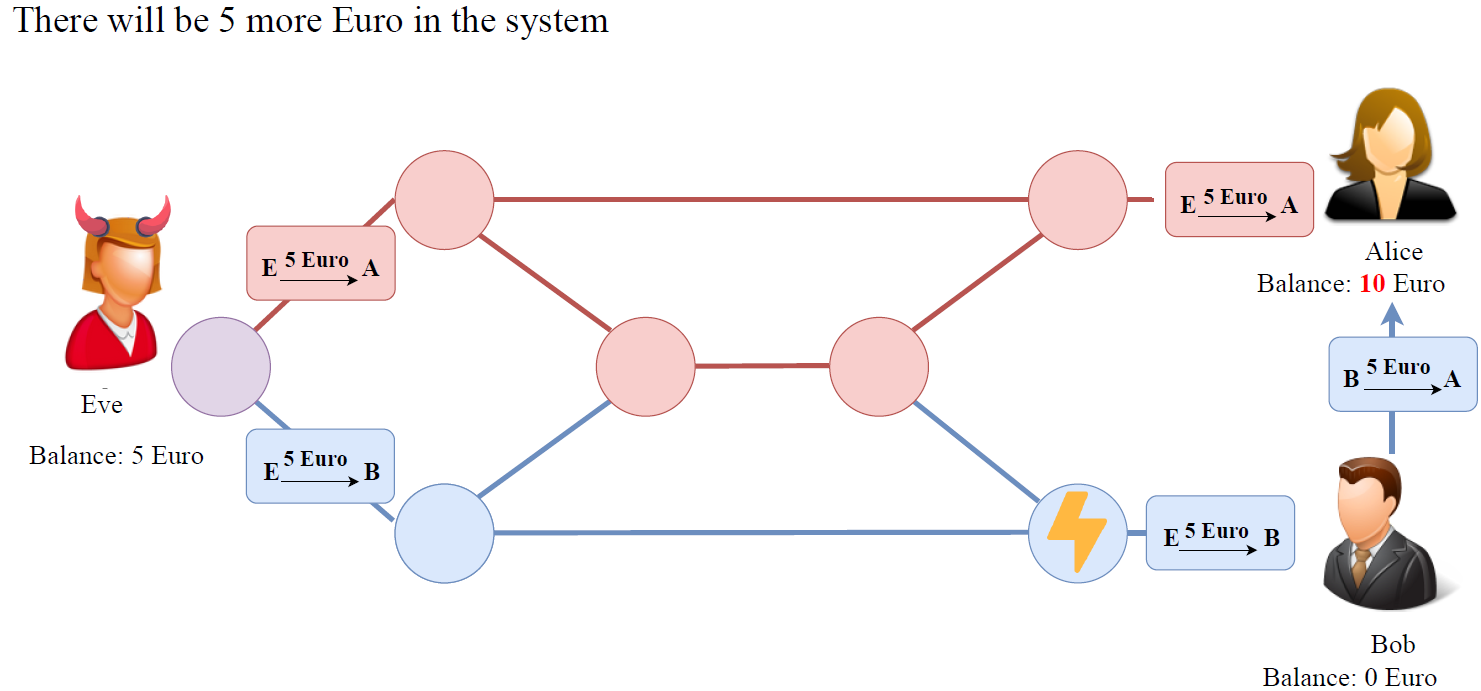
\includegraphics[width=\textwidth]{charts/DoubleSpend}
	\caption{Alice and Bob received repeated transaction }
\end{figure}

In 2008, a paper "Bitcoin: A Peer-to-Peer Electronic Cash System", written by Satoshi Nakamoto appeared on a US mailing list. This is the very beginning of Bitcoin. It proposed a mechanism based on the peer-to-peer network, using proof-of-work to record the public history of a transaction
that quickly becomes computationally impractical for an attacker to change if honest nodes control a majority of CPU power.

The network timestamps transactions by hashing them into an ongoing chain of hash-based proof-of-work, forming a record that cannot be changed without redoing the proof-of-work.\cite{sn} Bitcoin brought together a set of  techniques to enable the distrusting entities to transact directly with a digital currency. The following several elements are very important to help build Bitcoin system.

\subsection{Peer-to-peer network}

 In a general client-server network, a server takes charge of preservation and operation of data while clients request the server for the access of data and resource. On the contrary, in a P2P network, all participating nodes (referring to computers, also called "peers") hold data respectively and create an autonomous network wherein data are requested, meaning that each node acts both of server and client. P2P nodes have significant or total autonomy from central servers.

P2P networking technology has contributed to developing a base for a complete distributed network and eliminating single point of failure in Bitcoin.

\subsection{Cryptographic hash function}
A Cryptographic hash function is any function that can be used to map data of arbitrary size to data of a fixed size. This mechanism is characterized by the fact that the same hash value is obtained from the same data but only a slight difference in the original data results in a completely different hash value.

It is extremely difficult to infer the original data based on a hash value (non-invertible feature). Taking advantage of such characteristics, this mechanism is used for the detection of falsification of data, and in the Bitcoin system, it is used for the verification and guarantee the continuity of blockchain data and the creation of blockchain through Proof of Work utilizing the calculation of hash value.

\subsection{Consensus Mechanism}
The distributed nature of the peer-to-peer network requires the members (nodes) in the network to reach a consensus which validates the new coming data blocks which contain transactions by following a set of rules. The rules are specified in the algorithmic design of the blockchain system and can vary depending on its nature, purpose, and underlying asset.

In Bitcoin system, participants begin to propose the transactions. Before a transaction is allowed to be added to the global ledgers, other participants (also called miners) in the network first verify the validation of the transaction by solving a computational problem, once it is solved, they propagate answers to other miners along with the block of transactions. The other miners will accept the solutions along with the block of transactions and add those transactions to the global ledger. The Bitcoin transaction process is explained in the Figure 2.2.

The Bitcoin system, uses "Proof of work" (PoW) algorithm to establish consensus. Other frequently are used algorithms like Proof of Stake(PoS),  Practical Byzantine Fault Tolerance (PBFT).

\begin{figure}[!htb]% order of placement preference: here, top, bottom
	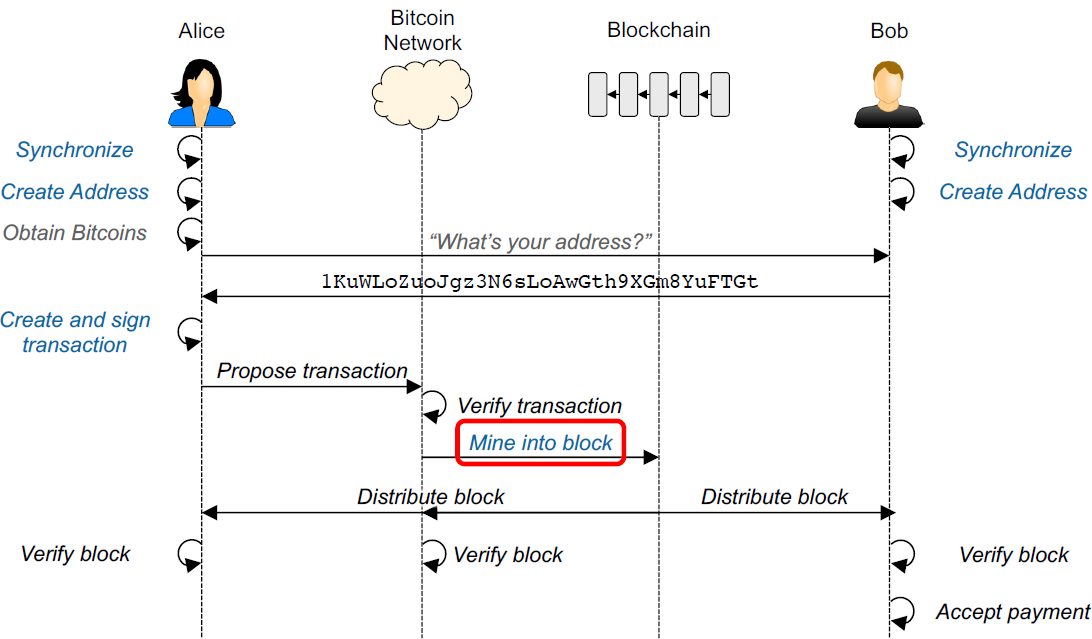
\includegraphics[width=\textwidth]{charts/BitcoinTx}
	\caption{Overview: Path of a Bitcoin Transaction\cite{sn}}
\end{figure}

\begin{itemize}
	\item \textbf{Proof-of-Work}
	
	Proof-of-Work (PoW) generally refers to a mechanism to confirm a node’s request for add a block (a block might contain several transactions) to the blockchain that involves solving a computational challenging puzzle in order to create a new block. PoW is also called mining in Bitcoin.
	
	\item \textbf{Proof-of-Stake}
	
	The Proof of Stake (PoS) algorithm is an energy-saving generalization of the Proof of Work algorithm. In PoS, the nodes are known as the "validators" and, rather than mining the blockchain they validate the transactions to earn a transaction fee. It based on the idea that the more stake of a node has, the more capable it can mine a block successfully. Thus nodes are randomly selected to validate blocks, and the probability of this random selection depends on the amount of stake held.
	
	\item \textbf{ Practical Byzantine Fault Tolerance (PBFT)}
	
	PBFT is an algorithm for solving a \textbf{Byzantine Fault} resulting from a failure in building a consensus caused by the Byzantine Generals Problem. Simply speaking, this algorithm ensures the consistency of consensus as long as two thirds of the network’s nodes are safe (i.e., not malicious or faulty). This is enabled by replicating behaviors (i.e., state machines) of generating nodes and applying protocols for choosing a leader among them. However,
	this method requires that all the generating nodes know each
	other since they need to communicate. In other words, all the
	parties have to agree on the exact list of participants.
	\cite{pbft}
	
	\item \textbf{Tendermint \cite{tendermint}}
	
    Tendermint is another byzantine consensus algorithm without mining work. It makes the assumption that the network is partially synchronized since the time factor is central to this protocol. For each new block, a validator node is selected in a round-robbin manner which has to propose a block. This block is then spread into the
    network and has to gather more than two thirds of votes of
    members within a given time period before being added to
    the blockchain. However, these members are selected based
    on their stake and thus ties trust to resource ownership.
\end{itemize}

\begin{table}[H] \centering 
%	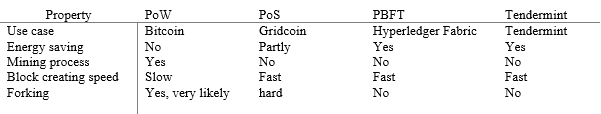
\includegraphics[scale=0.9]{charts/consensus}
     \ra{1.3}
     \begin{tabular}{{m}{3cm}ccccc}\toprule[0.5mm]
      Property & PoW & PoS & PBFT & Tendermint\\ 
      \midrule[0.3mm]
      Use case & Bitcoin & Gridcoin & Hyperledger Fabric& Tendermint\\
      Energy saving & No&Partly&Yes&Yes\\
      Mining process & Yes & No & No & No\\
      Block creating speed& Slow&Fast&Fast&Fast\\
      Forking& Yes, very likely&hard&No&No\\ 
      
      \bottomrule[0.5mm]
     \end{tabular}

	\caption{Typical Consensus Algorithms Comparison}
\end{table}
In the PoW the mining process is a brute-force approach, thus that is rather energy-consuming. While other algorithms without the mining process will be much more efficient. It also reflects on the speed of generating blocks. In the PoW, forking can happen if two miners find a suitable nonce at the same time. Meanwhile with
PoS, it is very difficult, happening only when a miner can own up to 51\% of all stake in the whole
verifying network. In the BFT-like consensus, e.g. PBFT and Tendermint, the validation essentially bases on the voting, it hardly forks.


\section{Blockchain Technology}
Blockchain originally came from Bitcoin's basic technology, referring a series of blocks created through PoW, and those blocks compiling transaction data for a certain period of time are linked into a chain. With the generalization of blockchain technology, it has more wide definition. Blockchain is a particular type of data structure used in some distributed ledgers which stores and transmits data in packages called "blocks" that are connected to each other in a "chain". Blockchain employs cryptographic and algorithmic methods to
record and synchronize data across a network in an immutable manner. \cite{WBank}

\begin{figure}[!htb]% order of placement preference: here, top, bottom
	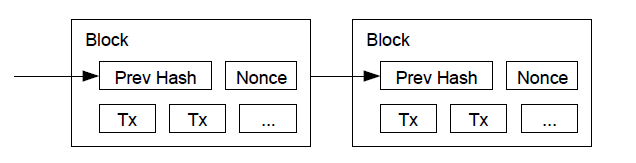
\includegraphics[width=\textwidth]{charts/blocks}
	\caption{blockchain appeared in Satoshi Nakamoto's paper}
\end{figure}

\subsection{Distributed Ledger Technology(DLT)}
Whenever the term blockchain is talked, frequently the related key word DTL would be mentioned.
Distributed Ledger Technology actually exists prior to Bitcoin, at least those techniques it represents are quite mature then. DLT is actually an umbrella term to the technology which is simply a decentralized database that is managed by various participants. Bitcoin blockchain is a milestone, which indicates the convergence of a host of technologies, including timestamping of transactions, Peer-to-Peer networks, cryptography, and shared computational power, along with a new consensus algorithm.

Distributed Ledger Technology generally consists of three basic components\cite{sawtooth}
\begin{description}
	\item [$\bullet$ A data model]that captures the current state of the ledger
	\item [$\bullet$ A transactions flow] that changes the ledger state
	\item [$\bullet$ A protocol] used to build consensus among participants around which transactions will be accepted, and in what order, by the ledger.
\end{description}
\textbf{Blockchain}, a particular
type of DLT, uses cryptographic and algorithmic methods to create and verify a continuously growing, append-only data structure that takes the form of a chain of so
called 'transaction blocks' – the blockchain – which serves the function of a ledger.\cite{WBank}

\subsection{Components of Blockchain system}
Having the foundation of Bitcoin's concept and DLT's structure, if we want to build a blockchain system, those components are likely required.

\begin{outline}
	\1 \textbf{Peer-to-peer network architecture}\\
	Due to the distributed nature, that each node in the network should keep a copy of the ledger. p2p network is the essential innovation shift to decentralized system.
	
    \1 \textbf{Consensus mechanism}\\
	As mentioned above, how consensus mechanism impacts the success of a blockchain system. It helps to validate the transaction, without the trusted third party.
	\1 \textbf{Smart contract}\\
	Smart contracts are simply predefined computer programs that execute actions when pre-agreed conditions within the system are met. Smart contracts provide the language of transactions that allow the ledger state to be modified. They can facilitate the business logic (e.g.  the exchange of shares, money, content, property). Smart contracts can be done in traditional centralized ledger systems as well, but the design of centralized ledger systems require such actions to be implemented only after the concerned parties have agreed to the underlying transaction as recorded in the central system.
		\2 \textbf{Decentralized Autonomous Organization(DAO)}\\
		A DAO can be seen as the most complex form of a smart contract, where the bylaws of the decentralized organization are embedded into the code of the smart contract, using complex token governance rules. At today’s evolutionary stage, a DAO materializes as a smart contract – a piece of code – executed on top of an increasingly opaque stack of distributed networking and consensus technology like the Ethereum blockchain or similar blockchains.\cite{dao}
	
	\1 \textbf{Cryptography}\\
	Cryptography has a key role to play both in the security, as well as in the immutability of the transactions recorded on blockchain . Cryptography is the study of the techniques used to allow secure communication between different parties and to ensure the authenticity and immutability of the data being communicated. For blockchain technology, cryptography is used to prove that a transaction was created by the right person. It is also used to link transactions into a block in a tamper-proof way, as well as create the links between blocks, to form a blockchain.
	
	
\end{outline}

\subsection{Types of Blockchain System}
Blockchain systems can be categorized as permissionless and permissioned. \textbf{Permissioned blockchain system} means that the parties that join the network are authenticated and authorized by an entity or
an administrator of the ledgers to participate on the network. while in \textbf{permissionless blockchain systems}, there is no central owner who controls network access. All that is needed to join the network and add transactions to the ledger is a server with the software.
The detailed comparisons are in the following Figure 2.4.\\
\begin{figure}[!htb]% order of placement preference: here, top, bottom
	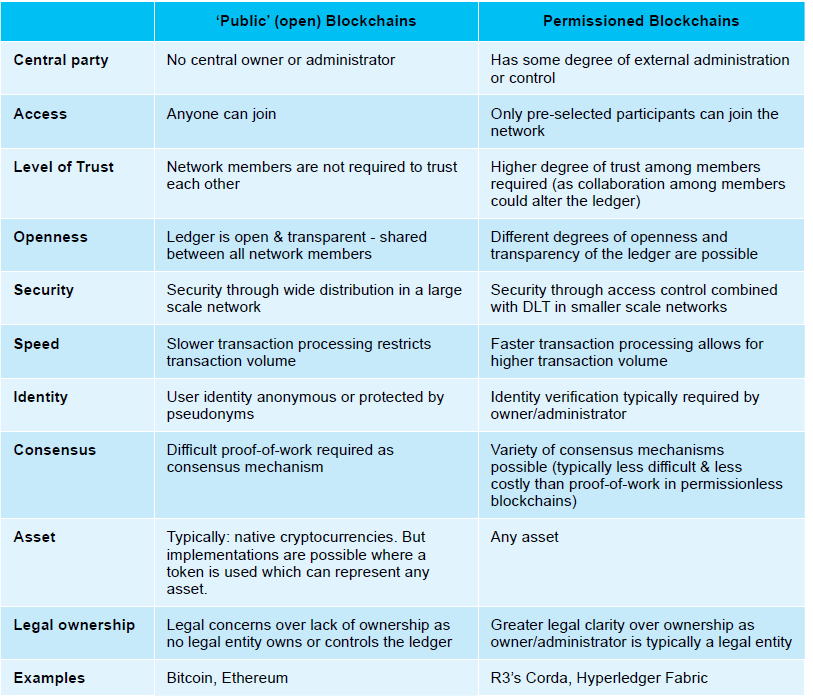
\includegraphics[width=\textwidth]{charts/permission}
	\caption{Comparison of permissioned and permissionless DLT}
\end{figure}
In permissionless blockchain systems, like the Bitcoin or the Ethereum, anyone can join the network, as well as write and read transactions. The actors in the system are not known, which means there could be some malicious actors within the network. Permissioned blockchain reduces these security risks and ensures that only the parties with valid identification can transact. 

There are several examples which base on the essential blockchain concepts and establish customized blockchain systems, which provide developers and companies with the architecture, where they can develop their own Dapps (Decentralized Applications).
  
\begin{itemize}
	\item \textbf{Ethereum} is an open blockchain platform(permissionless) that lets anyone build and use decentralized applications that run on blockchain technology.\cite{EthereumWhitePaper}  As the most popular blockchain for smart contracts, it facilitates the scripting functionality, or smart contracts which are run through the nodes in the network.
	\item  \textbf{Hyperledger Fabric} is a permissioned blockchain framework and one of the Hyperledger projects hosted by The Linux Foundation. Intended to create enterprise grade, open source, distributed framework for developing applications or solutions with a modular architecture. 
	\item  \textbf{Corda} is permissioned platform developed by R3 in collaboration with over 200 technology and industry partners. Smart contracts allow Corda to do this using complex agreements and any asset type. This capability has broad applications across industries including finance, supply chain and healthcare. 
	\item \textbf{IOTA} refers not only a cryptocurrency, but also a platform that entails a generalization of the blockchain protocol (the technology called Tangle) that sits at the backend of the IOTA platform. It enables machine-to-machine (M2M) transactions, which enhances the use of connected devices or the Internet of Things.
\end{itemize}

\subsection{Application of Blockchain Technology}
Deriving from Bitcoin, blockchain technology has a breadth of potential applications beyond cryptocurrencies in the financial field and in a wide variety of other industries.

According to World Bank's white paper, The two biggest trends in the development of blockchain applications are: 1) commercial Fintech start-ups are developing digital applications for a variety of purposes that utilize the public blockchain infrastructure, mostly Bitcoin and Ethereum;  2) industry consortia are forming to research and develop private, permissioned blockchain to solve industry-specific enterprise solutions. Actually the blockchain technology has been widely tried, in 2016 Nomura Research Institute have alreday conduct a survey on Blockchain Technologies, it visualized those applications based on Blockchain.
\begin{figure}[!htb]% order of placement preference: here, top, bottom
	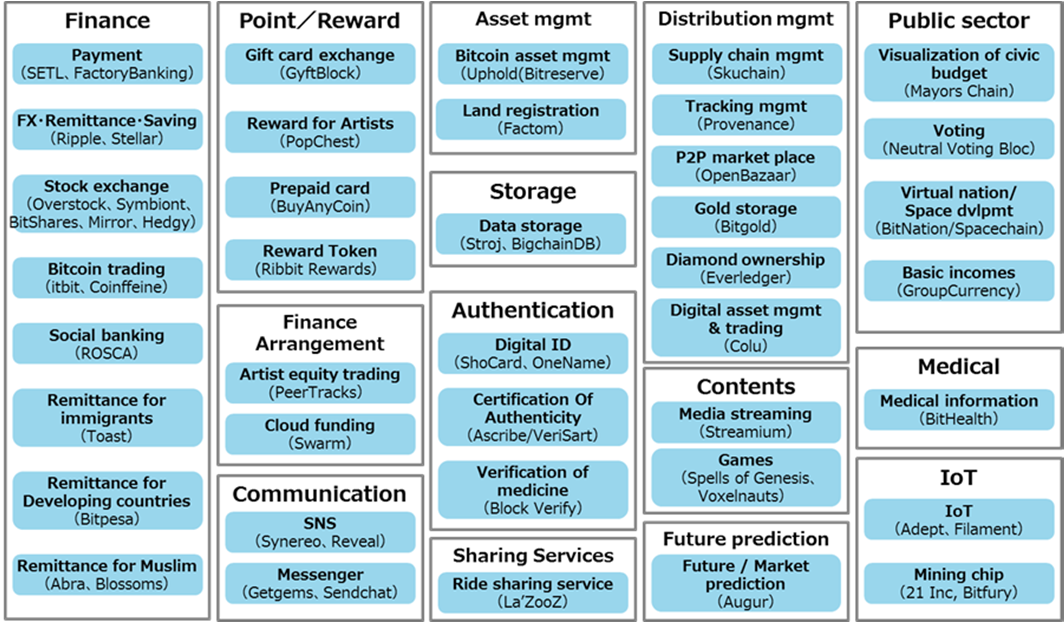
\includegraphics[width=\textwidth]{charts/Fields}
	\caption{Use cases and exmaples of services using blockchains\cite{JapanS}}
\end{figure}

\begin{itemize}
	\item \textbf{Finance}\\
	Ripple is one of the representative blockchains in this field.
	\item \textbf{Loyalty points and reward}\\
	GyftBlock, which provides an exchange service of gift
	cards using a blockchain.
	\item \textbf{Funding}\\
	Swarm provides a service to procure funds through cloud funding on a
	blockchain.
	\item \textbf{Communication}\\
	Messaging services and social networking services (SNS) have been
	made available using blockchains.
	\item \textbf{Asset management}\\
	Factom, etc. commenced the provision of a service.
	\item \textbf{Storage}
	Storj provides a service to manage various electronic files using a blockchain. Similar application like BigchainDB.
	\item \textbf{Authentication}\\
	uPort is a self-sovereign identity and user-centric data platform. 
	\item \textbf{Sharing}\\
	LaZooZ aims to provide a sharing service using a blockchain. At present, it provides a ride sharing application like Uber.
	\item \textbf{Commercial distribution management:}\\
	Everledger provides a system to manage
	diamonds. The serial number and carat, various commodity information, ownership and distribution record of each diamond are managed.
	\item \textbf{Content}\\
	Streamium provides a service to support content delivery, having established a system to charge by the second (paid with bitcoins) for video delivery, etc.
	\item \textbf{Prediction}\\
	Augur provides a decentralized prediction market platform where participants cast votes on various events to predict the future through the wisdom of the crowd.
	\item \textbf{Public}\\
	Neutral Voting Bloc (NVB) is a service provided in Australia, advocating itself as a new political party.
	\item \textbf{Medical services}\\
		BitHealth aims to achieve its goal to enable users to safely check
	their own health records from anywhere in the world using a blockchain.
	\item \textbf{IoT}\\
	Such services as ADEPT by IBM and Samsung are attracting attention.
	
\end{itemize}



\chapter{Turnover box system}
Turnover box system, the term is unfamiliar to most of us, yet it tightly connects with our daily life. Narrowly speaking, turnover box system aims to track the delivery of boxes among the partners in a certain supply chain. Those turnover boxes are containers of fruits, vegetables,
agricultural product, etc. In this chapter, I'll present the State-of-the-art of the supply chain, and its demand, requirement and problem. Also transit boxes as foundation of the logistic chain, how the blockchain system could be leveraged to boost the process.

\section{Supply Chain Management(SCM)} 
Ixxxxxxxxxxxxxxxxxxxxxxxxxxxxxxxxxxxxxxxxxxxxxxxxxxxxxxxxxxxxxxxxxxxxxxxxxxxxxxxxxxxxxxxxxxxxxxxxxxxxxxxxxxxxxxxxx

\begin{itemize}
	\item \textbf{Connected}\\
Ixxxxxxxxxxxxxxxxxxxxxxxxxxxxxxxxxxxxxxxxxxxxxxxxxxxxxxxxxxxxxxxxxxxxxxxxxxxxxxxxxxxxxxxxxxxxxxxxxxxxxxxxxxxxxxxxx
	\item \textbf{ Collaborative}\\
Ixxxxxxxxxxxxxxxxxxxxxxxxxxxxxxxxxxxxxxxxxxxxxxxxxxxxxxxxxxxxxxxxxxxxxxxxxxxxxxxxxxxxxxxxxxxxxxxxxxxxxxxxxxxxxxxxx
	\item \textbf{Cyberaware}\\Ixxxxxxxxxxxxxxxxxxxxxxxxxxxxxxxxxxxxxxxxxxxxxxxxxxxxxxxxxxxxxxxxxxxxxxxxxxxxxxxxxxxxxxxxxxxxxxxxxxxxxxxxxxxxxxxxx
	\item \textbf{Cognitively enabled}\\
	The AI platform becomes the modern supply chain's control tower by
	collating, coordinating, and conducting decisions and next best actions across the chain in an
	automated and timely way. Certain exceptions would require human
	intervention, but most of the supply chain would be automated and self-learning.
	\item \textbf{Comprehensive}\\
	Analytics capabilities must be scaled with data and in real time and insights must be comprehensive and fast.
\end{itemize}

\section{Logistics}
Logistics, the part of supply chain management, is the process of planning, implementing and controlling procedures for the efficient and effective transportation and storage of goods including services and related information from the point of origin to the point of consumption for the purpose of conforming to customer requirements and includes inbound, outbound, internal and external movements.

In order to realize the digitalized and smart supply chain, the modern Logistics, as the very essential part of the SCM, cannot come without roboticized, automatized process, telematics, Big Data, Cloud-based system.  Especially, the transport tool, that is, Turnover box draws the attention from companies, which are engaged in optimized the logistic process.

\textbf{Turnover Box}
- It is also called logistics box or transit box (hereinafter called the 'Box' also). In the Information age, it represents not purely the container of the goods, but integrates the relevant states, identity, channel, etc information.  

Thus Lufthansa Industry Solution proposed to setup a cloud-based platform integrated with logistics boxes, so that the clients can better track, check the goods, faster routing planning help to reduce the cost.\cite{lufthansa}

\section{Turnover Box System}
Why we focus on designing, developing and evaluating the Turnover Box System based on blockchain? Not only because several exploration in this specific field expands and even successful use cases come out from enterprises like Lufthansa, IBM, Deloitte. But also inspired by a client, who operates a company providing Boxes to the participants (For example, agri-food suppliers, goods distributors, product retailers) in certain supply chains, wanted an efficient, fault-tolerant, integrated system based on blockchain to help operate, manipulate and trace the Boxes and the cash flow. 

Thus this thesis, standing from the perspective of a Turnover Box operator, will depict, develop a digitalized, effective, easy access blockchain-based system, and evaluate whether the blockchain platform fits well in this scenarios.

\subsection{Challenges}
Digitalization in Business is changing the way we conduct business, the way we communicate, transact and interact with customers. And they tightly depend on their supply chain. As clients demand more transparency, the complexity of supply chains increases. An effective and inexpensive way to trace each material used in the final product is important in building confidence with increasingly environmental and socially conscious consumers. 
In sum, we list out the most concrete challenges when building such a versatile system:

\begin{itemize}
	\item \textbf{Transaction Throughput}\\
		The latest statistic shows that in recent 5 years every German consumes approx. 70kg fruits and approx. 98kg vegetables per year\cite{obst}. If we only take the city Düsseldorf with 660,000 people as an example, and only consider the consumption of fruits and vegetables, the whole city may need almost 1,1000-1,2000 Boxes (most common Boxes with 25kg load capacity) per day to deliver. So if we count in other agricultural products, and larger supply chain network in other cities, the pressure is obvious. Such huge volume of transactions and data must be proceeded efficiently.
		
	\item \textbf{Scalability}\\
		For a striving company, its business extends rather fast. While they add new partners, nodes and peers into their network, they also don't want the expansion obviously affect the user experience. And it also helps maintain the longevity of the blockchain (which is also essential for a supply chain). In the KMPG's latest report Demand-driven supply chain, they ranked the scalability as the third place.
	
	\item \textbf{Confidentiality}\\
		In real commercial world, the transaction confidentiality is sometime essential and useful. e.g. the operator want to take different price strategies among its clients, or in order to protect the data privacy of the product suppliers, the data confidentiality of the transaction really matters.
	
	\item \textbf{Robustness}\\
		For such a supply chain with various parties and transaction especially concerning payment, it is required that the system tough, dependable enough. The single-failure(usually happened in centralized system) should be avoided, to say least, the broken down or defected system(ledger) should be recovered easily. And it's also the reason we adopt the blockchain to track the flow.
		
	\item \textbf{Data Transparency}\\
		Not necessarily suitable for our Turnover Box System, but in Supply Chain becomes an increasingly significant elements. Specially in food supply chain, the source of raw material, producers, transport methods, expiration date are the focus of management to ensure food safety. Accordingly it helps to build more trustful cooperation among partners.    
\end{itemize}


\section{Key advantages of blockchain over traditional systems}
We chose blockchain technologies  as the basis to rebuild our digital supply chain system, because we did realize the challenges we faced, and recognized the features of blockchain which is immutable, transparent, and redefines trust, enables secure, fast, trustworthy, and transparent solutions that can be public or private.Those features surpass many traditional centralized ledgers or systems. The following lists shows the details:

\begin{itemize}
	\item \textbf{More Autonomy}
	
	 In blockchain-based system, every node plays roles as both of clients and servers. Nodes can submit the transactions at anytime. And the acceptance of the transaction depends on the counterparties and consensus algorithm. While the nodes in the centralized systems (traditional client-server mode) have to submit the proposal to the central server waiting to be proceeded. The way of submit transaction is much more autonomous.
	 
	\item \textbf{Higher Throughput} 
	
	As explained above, each node is both a client and a server. So many transactions submission and processing can run in parallel, which reduces the congestion in the network, improve the overall throughput rate.
	 
	\item \textbf{Automation}
	
	Smart contracts transfer the business logic into the programmed code. When similar business happens, the pre-set program will be triggered to proceed a set of actions.
	
	\item \textbf{Faster Transaction Process}
	
	Distributed design helps to improve the use rates of computing resources, which helps to reduce processing time
	
	\item \textbf{Robustness}
	
	Blockchain system basically avoids the "single failure" problem, which is the pain point of the tradition systems.
	
	\item \textbf{Immutability}
	
	In blockchain system, each entity must have assurance that their copy of the ledger is identical to other participants. This is the only way it can assure itself that the transactions it participates in are valid and unique. Malicious user must change record on all the ledger in the network simultaneously if it wants to tamper the ledger. 
\end{itemize}

\begin{comment}
	\item IBM cooperates with Walmart aiming to create a fully transparent food safe system \cite{walmart}.
	\item Oliver Wyman provides an End-To-End Blockchain enabled Supply Chain.
\end{comment} 


%(blockchain ubiquity)
Thus blockchain could be used to address inefficiency, lacking transparency and visibility, etc in current systems. Blockchain’s distributed ledger offers a means for exchanging assets in an open, secure protocol, which has interesting. To be more specify, how those issues are settle and how well they would perform will be our focus in this thesis. 

Thus it is promising but also challenging to build supply chain capabilities with the aid of blockchain which can result in greater levels of performance. 




\chapter{Design of the System}
As described in the previous chapter, the Turnover Box as very fundamental part of supply chain is the optimal experimental object to apply the blockchain technlogy. Before the development, this chapter will give an overview of the project design. It starts with the analysis of user requirements, then transfers the business model into conceptual model, in the end is the software and system design.


\section{Project description}
A Turnover Box system owner wants to implement an efficient, safe, automatically integrated comprehensive system to operate, control and manipulate the Boxes transactions with its cooperators.
\subsection{Product}
At end of the project, the Boxes operator, also as the owner will receive a blokchain-based system, on which all participants can do deal with Boxes. Only the owner can issue(add) new Boxes into the ledger as well as remove them.
\subsection{Roles}
In our scenario, there are mainly 4 roles:\\
\textbf{Box operator}: provides all types of the Boxes for delivering various products.

\textbf{Product Suppliers}: consume the Boxes as containers to transport various products.

\textbf{Distributors}: purchase the products from suppliers and then distribute them to different retailers. If received empty Boxes from retailers, the distributors should return those Boxes to the operator.

\textbf{Retailers}: order products from distributors and return the boxes either directly to operator or distributors. 

\bigskip
Figure 4.1 has clearly illustrate us how the participants in this network interact with each other and the flow of Boxes.
\begin{figure}[H]% use[!htb] to force the latex ignore the defaut
	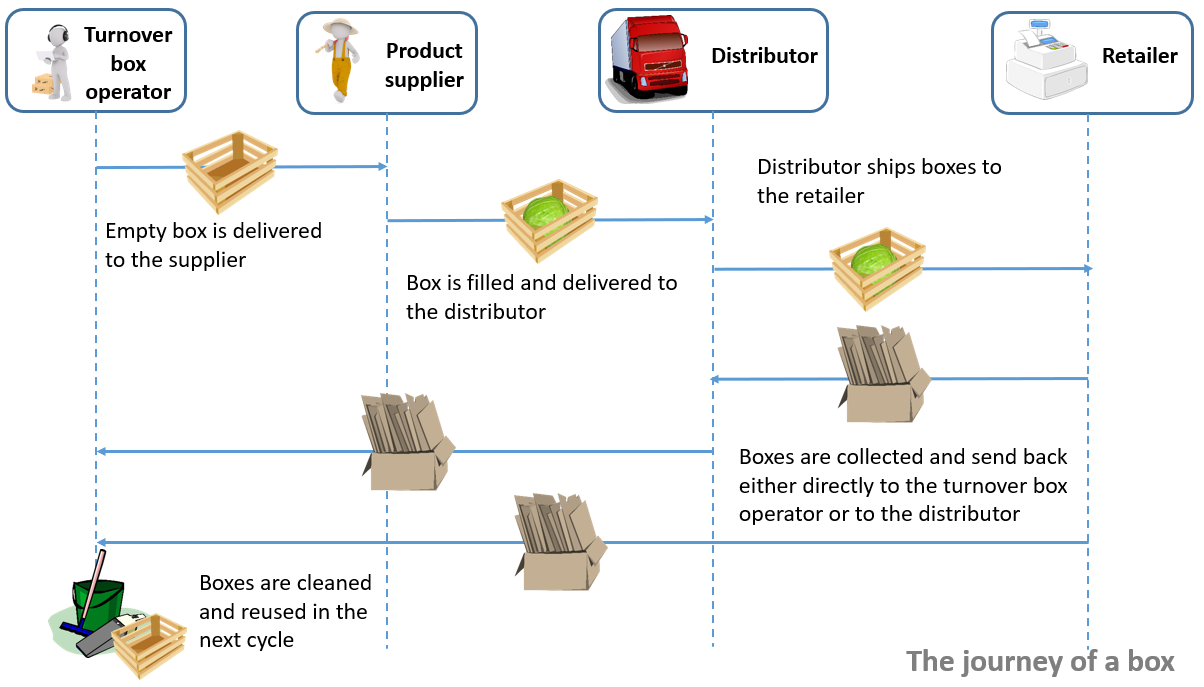
\includegraphics[width=0.9\textwidth]{charts/boxflow}
	\caption{The activity flow}
	\label{fig:label}
\end{figure}

\subsection{Pre- and post-conditions}
\subsubsection{Precondition}
\begin{itemize}
	\item There are two types of digital assets: Cash and Box.
	\item The number of Boxes should be positive.
	\item Participants' account should be positive.
	\item In the initial system, all participants' account should be zero.
	\item The Box has atomicity feature, which can not be partly treated.
	\item The Cash can be in any existing type of currency.
\end{itemize}
\subsubsection{Postcondition}
\begin{itemize}
	\item Ultimately, the income of the operator equals the outcomes of the suppliers and potential the rest of parties.
	\item Any parties who cause any damage to the Boxes should pay for the damage.
	\item There shouldn't exist any direct transaction between suppliers and retailers 
\end{itemize}

\section{Conceptual model}
A conceptual model is sufficiently comprehensive so that it can serve as a specification for developing software or a program, namely the simulation program. Setting up a conceptual model can help us
better understand the requirements, optimized the develop process, communicate with all parties involved and evaluate.
The conceptual model consists of a set of
components: the objectives, inputs, outputs, content, assumptions and simplifications of the model. 

According to the activity flow and the requirement, we can depict the conceptual model as Figure 4.2
\begin{figure}[!h]% use[!htb] to force the latex ignore the defaut
	\center
	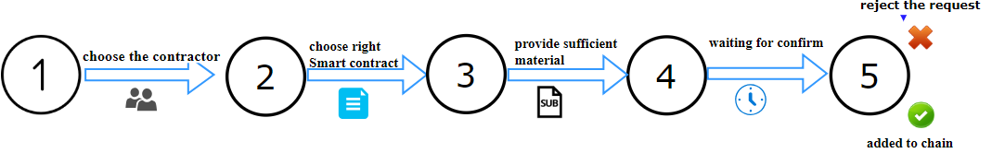
\includegraphics[width=1.1\textwidth]{charts/steps}
	\caption{conceptual model}
	\label{fig:label}
\end{figure}

In oder to have a better overview of the whole system, we draw the Figure 4.3. Participants can access the network through web or phone application.
\begin{figure}[!h]% use[!htb] to force the latex ignore the defaut
	\center
	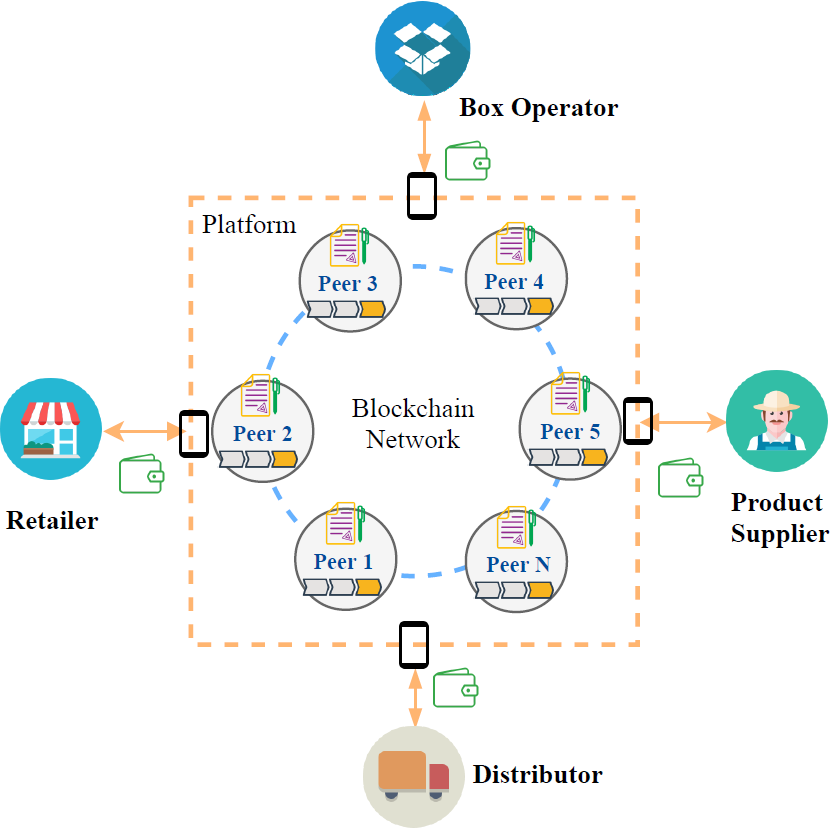
\includegraphics[width=0.9\textwidth]{charts/conceptual}
	\caption{overview graph}
	\label{fig:label}
\end{figure}

\section{Mapping into Smart Contract}

In the Figure 4.2, it demonstrates how the actual activities proceed.\\
We can also briefly conclude those mutual activities as following:
\begin{enumerate}
	\item Box operator \textbf{adds} new Boxes into the turnover box system.
	\item Product suppliers rent boxes from Box operator and \textbf{pay for the refuel fee}.
	\item Distributors purchase products from suppliers, and \textbf{pay for the pledge of the boxes}.
	\item Retailers place orders for products from distributors and \textbf{pay for the pledge}.
	\item Distributors and Box operator will \textbf{refund retailers the pledge} when retailers simultaneously restore the Boxes.
	\item Box operator \textbf{refunds distributors the pledge} when the Boxes are restored.
	\item Distributors \textbf{decide the box types} with Box operators. 
	\item Distributors require the supplier to use certain types of Boxes.	
\end{enumerate}
In sum, we want to translate the business logic into automatically executable program, that is called chain code or smart contract. Roughly now we could anticipate 5 main contracts.
\begin{itemize}
	\item \textbf{func addBox (boxinfo, ChaincodeStubInterface)}\\
		  The addBox function is the method turnover box Operators use to record of the new boxes coming into service. 
		  
	\item \textbf{func payforPledge(counterparties,Box.type, Box.num)}\\
	      The PayforFee method is the method actors use to pay for the Fee during the delivery.
	      
	\item \textbf{func damageCost(box.num, box.type)}\\
	      The damageCost method is designed to fine the party, which damages or loses the Boxes.
	      
	\item \textbf{func refund(counterparty, box.type, box.num)}\\
	      The Refund method is the method actors use to refund the Fee during the delivery. This contract should be similar to the payforFee method.
	      
	\item \textbf{func deposit(party, num)}\\
	      Recharge method is extremely crucial method in the supply chain, since the Hyperledger Fabric, and Corda has no token and wallet, so we devise Recharge method as a prepay contract, 
	      All the actors can only deposit at the turnover box operators. After recharging the deposit
	      can be written as digital assets store in the Blockchain
\end{itemize}




\chapter{Related Works and Application}
This chapter provides an overview over current blockchain applications in field of logistics and supply chain management both in academia and industry. Through analyzing the performance, feedback, research, it helps us prepare for the next implementing step. Last but not least, I will present the preparation for setting up the application, especially the consideration on how to choose the right platform.

\section{Research in the Scientific Community}
Since 2017 the amount of research papers discussing the possibility of applying blockchain technologies into logistics field have witnessed a sudden blowout. It draws great attention from academical world. 

In 2017, Finnish researchers haven dived into the integration blockchain into Digital Supply Chain (DSC), they pointed out that traditional integration of DSC seemed to be a significant gap in many functionalities. This was an interesting finding, as intermediates (EDI operators)including banks (SWIFT operators) have been operating and collaborating in this area over two
decades, but services still lack some fundamental
functionalities (e.g. standards, timestamping of
transactions, monitoring and tracking of information
flows and secure end-to-end delivery of information).An analysis showed many of these missing
functionalities to be embedded in blockchain technology.\cite{chapter4-dsc}

Researchers from China attempt to address the agri-food safety problem through optimizing the food supply chain. They depicted a system using RFID and blockchain technology in building the agri-food supply chain traceability system, including production link, processing link, warehousing management link, cold chain distribution link, Sales link. When consumers are shopping in the supermarket, they can use the
RFTD reader to obtain the basic infonnation of agri-food
products by scanning their RFID tags. All the information along the agri-food supply chain is fully realtime auditable in blockchain.
Transparency of products information could significantly
enhance the consumers' trust for products and obviously
increase their confidence for the agri-food markets.\cite{chapter4-RFID}

Remarkably researchers from Portland University proposed a block-supply
chain, a new decentralized supply chain that detects counterfeiting
attacks using blockchain and Near Field Communication (NFC). Their simulations show that the proposed protocol offers remarkable performance with a satisfactory level of security compared to the state of the art consensus protocol Tendermint.\cite{chapter4-nfc}

\section{Trial in Industry}
From any perspective, the industry field is always the first one to perceive the great potential and chance laying in blockchain.
Indeed some enterprises are actively trying out the exploration. There we can have a look at the those applications from different perspective.

\subsection{Classification}
There exists several criteria can be used to classify blockchain applications. Therefore we try to list the as complete critertia as we can to provide better view of the applications.
\subsection{Products or Platforms}
Blockchain applications can be categorized into two camps: product-oriented or platform-oriented. The distinct also shows in the the business models they run. The product-oriented applications is B2C model which provides clients the blockchain-based solution in specific scenarios. The example are like uPort mentioned in the previous chapters, controls the users' ownership of identity. Another type is the
platform-oriented, which is more familiar to most of blokchain developers. The second type usually provides open sourced platform, aiming to setup the field standard, and gradually to build a ecosystem. Hyperledger Fabric and Corda are the latter type, which have wilder ambitions.

\subsubsection{Assets and Token}
First and most of second generation of blockchains like Bitcoin or Ethereum, have native tokens (or Cryptographic Tokens, Cryptocurrency). 
Token are part of the incentive scheme to encourage a disparate group of people who do not know or trust each other organize themselves around the purpose of a specific blockchain. And the new generation of blockchain like Corda and Hyperledger were designed to run with a single shared ledger among all network participants. This allows any participant to view all transactions, including those of competitors. While smart contracts provide an amazing leap forward in how blockchain can be applied to business transactions. 
%(blockchain ubiquity)
\subsubsection{Consensus Algorithms}
The Consensus algorithm has vast effect on blockchain systems' features. Especially the performance, whether it has mining process or not is the key issue. In chapter 2, we gave a precise introduction and comparison of consensus algorithms. The table will help readers to categorize the applications. 

\subsubsection{Business Scope}
While we described above the blockchain applications from a technology perspective, we can also use a commercial approach to map them. Since in different fields of usage, the requirement for security level, running platform, scalability,etc will be distinguishing. Also in the end of Chapter 2, we listed out a wide variety of applications in all kinds of areas.
\subsubsection{Open or Close Source}
For most of open source projects, their incentives are to provide a standard platform, which ultimately to create a ecosystem. And some close source projects attempt to protect the intellectual property, which sell the projects as product. This prospective of categorization is similar to the first one we mentioned above.
\subsection{Platform Benchmarks Overview}
Blockchain technology is recently under extensive research and development,
leading to a high market fragmentation. Until November 2018, according to incomplete statistics, there exists more than one hundred blockchain projects\cite{platforms}, we list the top 5 popular platforms with detailed description, also the Table 5.1 compares the key characteristics of the mature platforms. 

\begin{itemize}
	\item Ethereum \\
	Mature Smart Contracting Cross-Industry Platform. Ethereum Wallet that allows holding crypto-assets, and writing, deploying and using smart contracts. Making cryptocurrencies. Theoretically speaking, it is a generic platform for all kinds of transactions and applications. Concurrently it has obvious limitations ans shortness. It is PoW based which is not the fastest (resulting in potential latency issues) and is a massive energy consumer. Though it might change its consensus algorithm to the fast PoS in future versions.
	\item Hyperledger Fabric\\
	Hosted by Linux Foundation and launched in 2016, is an open-source collaborative effort to advance cross-industry blockchain technologies. One of its key goals is to create enterprise-grade distributed ledger frameworks and codebases. Hyperledger Fabric provides a modular architecture, which allows components 
	such as consensus and membership services to be plug-and-play. Hyperledger Fabric 
	leverages container technology to host smart contracts called "chaincode" that comprise 
	the application logic of the system
	\item Quorum\\
	An open source private Blockchain network developed by JP Morgan from the 
	Ethereum code. Quorum’s essential distinguishing feature is the fact that it allows private transactions between the parties. Ideal for applications requiring high speed and throughput processing of private transactions.  It does not use the Proof of Work (PoW) consensus algorithm but uses vote-based and other algorithms enabling it to process hundreds of transactions per second, depending on how smart contracts and networks are configured. 
	\item Corda\\
	R3 is a consortium of some of the world's biggest financial institutions that has created an open-source distributed ledger platform called Corda. A distributed ledger platform Like Hyperledger Fabric, it is a product designed from the ground up for enterprise networks, generally banks, finance. There is no built-in token or cryptocurrency for Corda, and it is a permissioned blockchain as it restricts access to data within an agreement to only those explicitly entitled to it, rather than the entire network. Its consensus system takes into account the reality of managing complex financial agreements. It is also known for its focus on interoperability ease of integration with legacy systems.  
	\item BigChainDB\\
	An open source system
	 that starts with a big data distributed database and then adds Blockchain characteristics - decentralized control, immutability and the transfer of digital assets. It focuses on the distributed database, so here we exclude BigChainDB from our project of development.
\end{itemize}
\begin{landscape}% Landscape page
	\thispagestyle{empty}% empty page style (?)
	%\centering % Center table

	\begin{table}[H] \centering 
		%	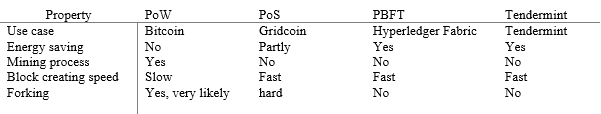
\includegraphics[scale=0.9]{charts/consensus}
		\ra{1.2}

		\begin{tabular}{{m}{3.5cm}cM{2.5cm}M{2.7cm}M{2cm}{m}{1.8cm}ccc}
		\toprule[0.6mm]
			Projects & Start year & Governance  & Popularity
			(GitHub stars)& Smart Contract & Consensus&Throughput &	VM&Oracle\\ 
			\midrule[0.3mm]
			
			Ethereum & 2015	&Ethereum Foundation& 21k&	Yes &PoW&15 tps& EVM&Yes\\
			
			Quorum & 2013&J.P.Morgan&2799&Yes& Voting&10+ to 100+ tps&EVM&-\\
			
			Hyperledger Fabric & 2016&IBM&7280 &Yes&PBFT& > 2000 tps& Docker&No\\
			
			Corda& 2015& R3 &2519& Yes& pluggable&~ 170 tps	&JVM&Yes\\
			
			BigChainDB&2013	& BigChainDB& 2992&	No&	Tendermint&N/A &Optional&Yes\\ 
			Monax &2014	&Monax&271&Yes&Tendermint&N/A&EVM&No\\
			Multichain&2015	&Coin Sciences	&441&No&PBFT,round robin, etc&100-1000 tps&No&No\\
			Ripple&2014&Ripple Labs&3k&	No&	Probabilistic Voting&0.25 tps&RVM&No\\
			
			\bottomrule[0.5mm]
		\end{tabular}

	\caption{Comparison of different blockchain platforms}
	\end{table}
\end{landscape}

\begin{comment}
\begin{landscape}% Landscape page
	\thispagestyle{empty}% empty page style (?)
	%\centering % Center table
	\begin{figure}\centering% order of placement preference: here, top, bottom
		
\includegraphics[scale = 0.23]{charts/benchmark}
		\caption{Comparison of different blockchain platform}
	\end{figure}
\end{landscape}
\end{comment}
\clearpage

\subsection{Criteria for platform selection}
As fully described and compared above, there are multitude of different blockchain platforms with specific functional incentives. How to choose the proper platform without getting overwhelmed in the sheer volume of potential techniques? Researchers from Fraunhofer FIT gave a set of criteria\cite{fraunhofer} for selecting the right one:
\begin{itemize}
	\item Access policy – Permissioned vs. public blockchain;\\
	In our case, considering the industrial confidentiality, permissioned platform is required, thus the Ethereum will not be taken into consideration.
	\item Process integration – Availability of smart contracts or
	chain code;\\
	Some projects provides a network for their native cryptocurrency, like Ripple and Multichain are not suitable here.  
	\item Scalability and transaction performance – Transaction
	throughput;\\
	This is extremely important in the industrial cases. In blockchain systems, we use "transaction per second (tps)" as the measurement for performance.
	\item Restricting data access – Data privacy and visibility;\\
	The first and part of second generations of blockchain, like Ethereum, were designed to run with a single shared ledger among all network participants. This allows any participant to view all transactions, including those of competitors. In our scenario,  we prefer platforms like Hyperledger Fabric and Corda which have confidentiality design.
	\item Network governance – Ease of adding/removing nodes
	to the network;\\
	Lightweight administration process should be encouraged, so that the join and exit of the network will not lead to shutdown of the whole system or reconfiguration.
	\item Technology governance – Open source, project
	management, development kits.\\
	The last criterion is also of major importance, because the technology governance will vastly impact your project's performance, stability, development process and success. Especially for open source project, 
	developers should better examine whether the future of the platform is guaranteed, i.e. whether the it is periodically and stably updated, whether the bugs are solved in time, etc

\end{itemize}
In sum, for the Turnover Box System, we need a permissioned blockchain framework, with usable and efficient method for digital asset, smart contract development. Hyperledger Fabric, R3 Corda, Quorum are all qualified open source options, however considering the unstable throughput of Quorum, we narrows the options only to the Hyperledger Fabric and Corda.

\subsubsection{Hyperledger Fabric vs. Corda}
\begin{outline}
	\1 Languages Support
		\2 Fabric support for: 
			\3 Go(since v1.0)
			\3 Node.js(since v1.1)
			\3 Java(since v1.3)
		\2 Corda support Java and Kotlin
	\1 Prerequisites for development
		\2 Fabric requires the tools to be installed:\\ 
			1. cURL\\
			2. Docker and Docker Compose\\
			3. Go version 1.10.x is required\\
			4. Node.js Runtime and NPM\\
			5. Python for Ubuntu 16.04 users\\
		\2 Corda uses industry-standard tools: \\
			1. Oracle JDK 8 JVM - minimum supported version 8u171\\
		    2. IntelliJ IDEA - supported versions 2017.x and 2018.x\\
		    3. Git\\
	\1 Database and Queryability
		\2 Fabric has a state database based on either \textbf{LevelDB} or \textbf{CouchDB}, both support key range queries
		\2 Corda uses a relational database for data storage, supports SQL  including H2, SQLServer, and PostgreSQL, can be direct accessed.
	\1 Platform support
		\2 Fabric supports most of the OS and architectures. And major cloud providers have embraced Hyperledger Fabric offerings (AWS, Azure, IBM, Oracle, SAP) 
		\2 Corda runs on the JVM, which can be used widely across different platforms. AWS, Azure are also supported.
     \1 Open Source and Governance
     	\2 Fabric is open source and governed by Linux Foundation. Hyperledger Fabric owns very big community, there are more than 140 contributors and 7000+ stars on Github. 
     	\2 Corda is  also open source governed by company R3. Comparing with Hyperledger, Corda's community is relatively small.
\end{outline}

When consider the developer friendly, precise documentation, performance, etc, it is hard to choose a platform from the two, if we let it remain theoretical. The best way is to try them out, and discuss in the conclusion part.

\chapter{Application}
In this chapter, the details of implementation will be discussed. It starts with an overview and the architecture of the blockchain enabled logistic application, and is followed by three important component in the application: transaction, the consensus, and the flow. In the next section, we provide a UML class diagram and several tables to describe the functionalities of the classes. However, all the structures and designs are based on the Corda platform. 

\section{Architecture}


\begin{outline}
	\1 Storage services and vaults backed by a SQL DB
	  \2 Default DB is h2  
	\1 RPC client framework and server shell for communication amongst network nodes
	\1 Customized functionality called CorDapps.
	   \2 States, Flows, Contracts are essential for CorDapps.
	\1 ServiceHub internal contains references to the 8 service features(in Figure 6.3, the 8 blocks beneath ServiceHub, except Storage Service)
\end{outline}

\begin{figure}[!htb]% order of placement preference: here, top, bottom
	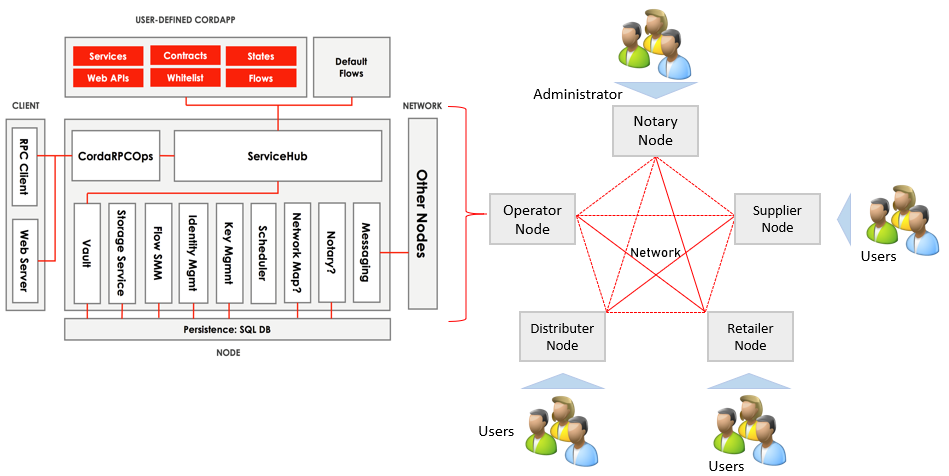
\includegraphics[width=\textwidth]{charts/node-architecture}
	\caption{The architecture of a single node}
\end{figure}

%=========================================================================
\section{Key Components}
This part provides in-depth information of about Corda's components, which helps audience better master the inner logic of the platform. It's critical for successful development.

\subsection{Roles in Corda}


\subsection{Corda Network}

	
\subsection{Corda Ledger}

\subsection{States}

\subsection{Contracts}

\subsection{Flows}

\subsection{Consensus}

%=========================================================================
\section{UML}
\subsection{Action Sequence}


Next Chapter we will demonstrate the performance and the correctness of our system.

\chapter{Test and Evaluation}
Software testing is an investigation conducted to provide stakeholders with information about the quality of the software product or service. It is very critical step in the process of software development. It plays especially a decisive role of the secure and successful blockchain application development. A single bug in a smart contract can open a security hole wide enough for someone to reach in and steal the entire contents of your digital asset.
\section{Testing Environment}
Corda uses industry-standard tools and running environment:
\begin{itemize}
	\item Oracle JDK 8 JVM - minimum supported version 8u171
	\item IntelliJ IDEA - supported versions 2017.x and 2018.x (with Kotlin plugin version 1.2.51)
	\item Git
	\item database h2
	\item OS: Windows 10 and IOS
	\item Memory: 3GB RAM
	\item CPU: Intel 2 cores.
	
\end{itemize}

\section{Functional Test}
In order to ensure the correctness and validation of our project, taking functional test turns out to be absolutely critical and necessary. Further more, this part will vastly assist readers better understand the process and mechanism. In this section, Unlike the usual software development documentary, only the core functions  and carefully selected test cases will be presented. 

\subsection{Function 1: Add Box}


\subsection{Function 2: Deposit}

\subsection{Function 3: Refuel Fee}

\subsection{Function 4: Pledge}


\section{Integration Test}
After the unity and functional tests, Integration Test cannot be omitted, since it ensures that the integrated modules/components work properly, and detect the interface error.

In order to complete the test, we divide the whole test as following steps which was illustrated in the Figure, 
\begin{figure}[H]% order of placement preference: here, top, bottom
	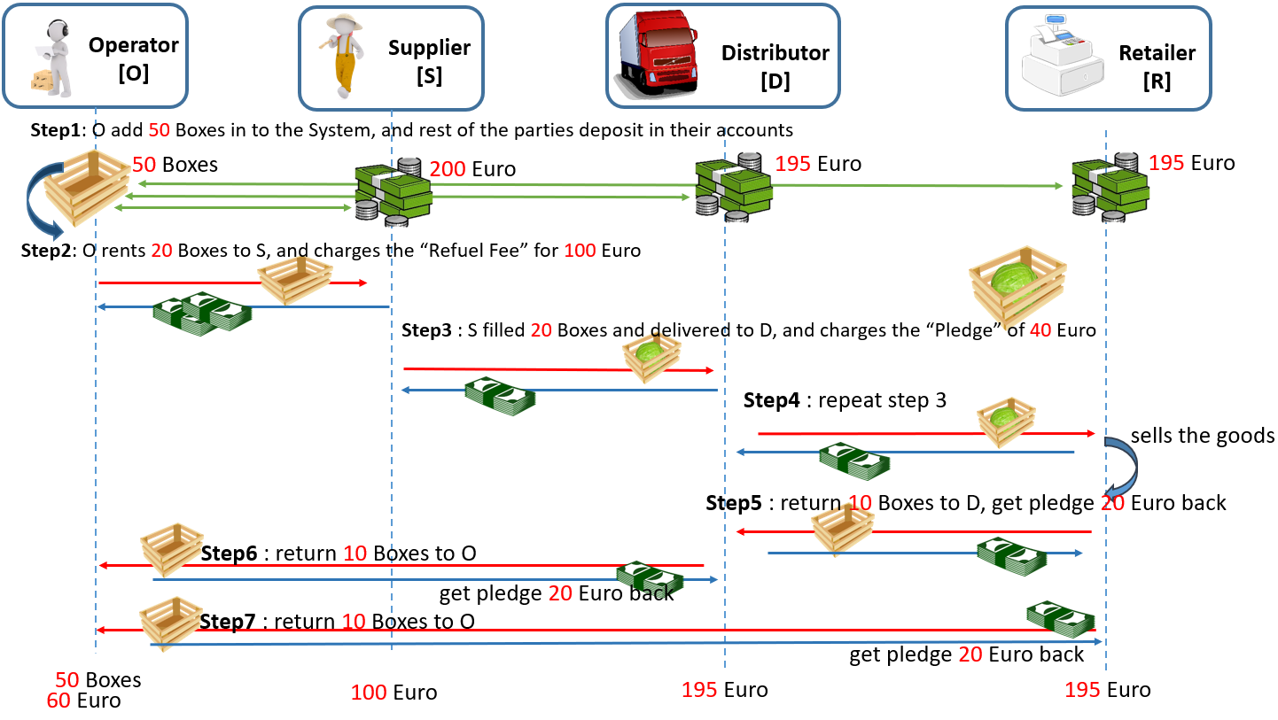
\includegraphics[width=\textwidth]{charts/c7-test-overview}
	\caption{The Cash and Box flow of PledgeContract}
\end{figure}



% ==================Performance=========================
\section{Performance Test}
Performance test plays a crucial role in our project. Whether leveraging the blockchain technology depends on how well and reliable it runs in reality. In this section, the expected features like high throughput, robustness, synchronization, etc are tested. 

However the Performance is multi-dimensional, multi-variable issue. In our cases, the performance highly relates to the following factors:
\begin{itemize}
	\item \textbf{Complexity of Contract and Flow.}\\
		The contracts and Flow contains the actual business logic, boundary conditions, and constraints. The more complicated they are, the slower performance would be. So it also provides us with the insight why and how we should optimize the program. Like in this project, the "Addbox" transaction in most cases is much faster than the "Refuel Fee" contract.
    \item \textbf{Consensus and Notary Type}\\
        The very classic argument is about the speed of "POW" and "POS", different consensus will vastly influence the performance. In Corda, it is via Contract's verification function and Notary' investigation to do the work.
        In our prototype, since the Corda blockchain doesn't have token, so the users have to transfer money offline; and because of no external reference, the Operator have to manually confirm the deposit from users.
    \item \textbf{Network and Infrastructure}\\
		This is quite important feature for any network-based application. For nodes running on local infrastructure, the number of cores, the CPU, the database.
\end{itemize}
\subsection{Throughput}
One of the core criteria when we estimate the system' performance. Taking the simplest transaction "AddBox" and the most complicated transaction "Pledge" as the test sample.

\subsection{Robustness and Recovery}
The stability and robustness of our system are estimated in the following perspectives.
\subsubsection{Node data storage}

\subsubsection{Recovery from node crashes}


\subsubsection{Recovery from corruption/deletion of the node's files}


\section{Features of this Project}
Though the previous steps have clearly demonstrated the functional features. However there are other characteristics of this Corda-based application, which need to be highlighted. It would be the very first-hand material and direct reference of people want to setup an analogous project. 

\subsubsection{Identifiable Participants and trustworthy counterparties}

\subsubsection{Multi-User and multiple permission}

\subsubsection{Pluggable Notary services}
 
\subsubsection{Multiple notaries}
 
\subsubsection{"Need-to-Know" mechanism}

\subsubsection{Confidentiality}

\section{Future work}



\chapter{Result and Conclusion}
Looking back through the thesis, What was researched, compared, investigated, designed, developed, and estimated are now exceeding the completion of a blockchain-based application. During the process of whole research, I have been constantly inspired to think various problems far beyond the project itself. So in this chapter, it was constructed by my insights, thoughts, and Outlook.

\section{When to Use Blockchain}
Like Maslow once said "if the only tool you have is a hammer,to treat everything as if it were a nail." In the software industry we repeatedly find new and cool hammers and then try to hit as many nails as we can. And the new one now is Blockchain. Today the media a little bit exaggerate the capability of Blockchain technologies, you can easily find out massive blockchain-embedded solution in many field. However blockchain isn't panacea, thus it is necessary to evaluate if blockchain technology is right for a particular project.

\subsection{Factors to Consider}
So before any enterprise makes up their mind of adopting Blockchain techlogies, it is necessary to conduct a comprehensive estimation whether applyin Blockchain or not. Hyperledger Technologies Organization gives generalized, high-level decision points about when to use or not to use blockchain technology (Figure 8.1)
\begin{figure}[htb]% order of placement preference: here, top, bottom
	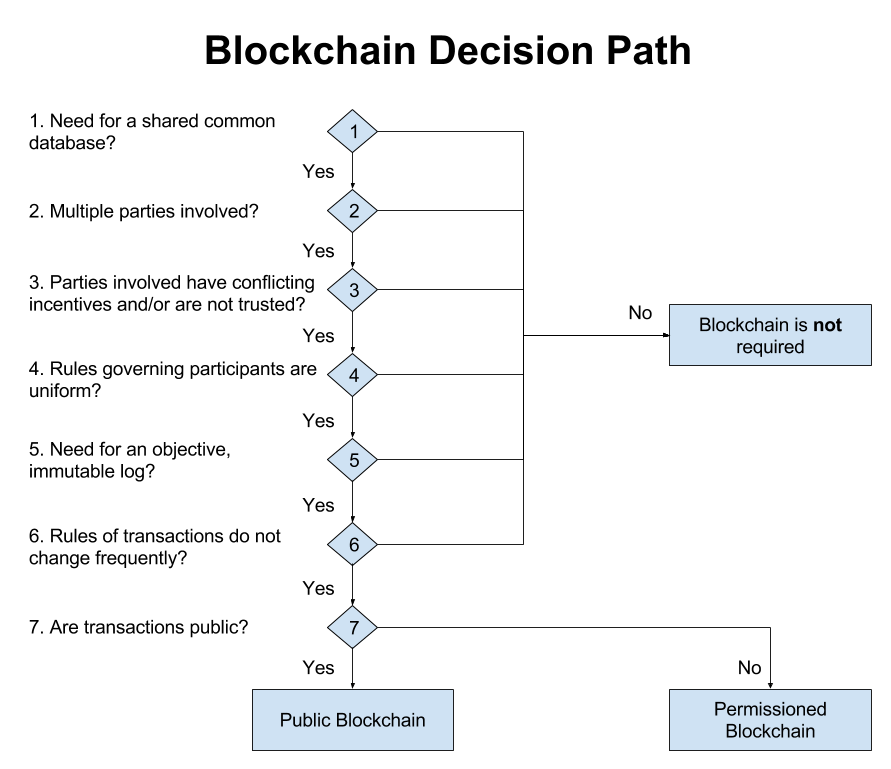
\includegraphics[width=\textwidth]{charts/Blockchain_Decision_Flowchart}
	\caption{Blockchain Decision Flowchart \cite{decision}}
\end{figure}
Comparing with when is suitable for using blockchain, when is \textbf{NOT} requires our caution more. Those are some conditions which are not suitable to develop blockchain-based soltions:
\begin{itemize}
	\item Business logic changes frequently\\
		- The smart contract is pre-set in the Nodes, frequent change may cause the failure of the system.
	\item Strict confidentiality\\
		- In the permissionless Blockchain platforms, the data is transparent to anyone. Even permissioned Blockchains with special mechanism to increase the privacy, like Corda and Hyperledger Ledger, the data is still at least known to the involved parties. Business with low tolerance for data transparency is not suitable for using blockchain. 
	\item Large Data Exchange \& Storage \\
		- In Blockchain system, the ledgers are fully or partly(like Corda) stored in each Nodes. The rate of repetition is rather highly, thus it is suitable for systems only storing the minimum necessary information, without too much data exchange in each transaction.\\
	\item Better alternatives\\
		- If there exists simpler, more mature options, it would be more effective.
\end{itemize}
 
\section{Summary}
The 6-month master thesis is until here almost to an end. It all stared with an occasion that 5 years ago I stumbled upon the term "Bitcoin", and later I got to have deeper insights about the blockchain technology. However, it took quite considerable time to find the satisfying research orientation. Yet it was only the tip of an iceberg, during research and development, there always sprang up unexpected challenges, and countless hours with effort were invested. In retrospect, considering the obstacles overcome, the result achieved, and the valuable reference information provided, all the work was worthwhile.

\subsection{What Were Accomplished}
The master thesis started from doing research about how far have the applications of blockchain technology proceeded in diverse fields, how practical they are. Among the wide range of fields, the application in supply chain has been chosen to be the object of study.
Logistics is a very important part of supply chain, it controls the delivery ability and circulation. To be specific, how to manage the Turnover Boxes efficiently, robustly, transparently and automatically is the core issue. Thus using blokchain as the tool to solve the pain point.\\

Before I started the project, I have been dived into the blockchain platform pool aiming to get the first-hand information for the application. In the end, the two candidates: Hyperledger Fabric and Corda haven been chosen to realized the Turnover Box System. The purpose was to find out the best suitable platform to build the Turnover Box System, and provide first-hand information for the companies having the similar business logic to help them build their own blockchain applications\\

After 3-4 months development, the CorDapp has successfully come into use, which works as well as expected before. The developing plan on Hyperledger Fabric has been pruned. In the previous chapters, the details of design, development, test and evaluation on this CorDapp have demonstrated Corda is the optimal choice for the Turnover Box System.\\

 
\subsection{Why Corda not Hyperledger Fabric}
Though in the previous chapter, the comparison between Hyperledger Fabric and Corda has been listed. Those differences are only from the theoretical analysis. After the involvement in both platform, there are some reasons why the Corda is more suitable than Hyperledger Fabric from the developers' perspective.
\begin{itemize}
	\item Higher Prerequisites \\
	- Hyperledger Fabric requires more dependencies, the smart contracts ("chaincode") run within a container environment(e.g Docker). Usually a single wrongly installed version of the tools will cause errors.
	\item Complex configuration \\
	- in order to set up the Hyperledger Fabric network, Hyperledger Fabric platform-specific binaries, docker images should be installed. The docker configuration file is rather tedious and no clear clue to guide.
	\item Unstable version update \\
	- Usually when a new version of the platform arrives, most of previous dependencies won't work at all and need to be updated. The docker images' frequent changed locations will also cause a lot of "Not Find" errors.  
	\item Bad Documentation \\
	- Frequent change but slow update in documentation, which usually results in the invalid links on the web page. No precise guidance in configuration and development.
\end{itemize}
Comparing with Hyperleger Fabric, the corda is relatively compact, flexible and efficient with reduced prerequisites, dependencies and usage of JVM.

\section{Outlook}
Today the blockchain on the one hand has been highly praised, on the other hand has been taken as hype suspect. After having had a close touch with it, I prefer to see the more positive side. The call for lower-cost management, traceability, transparency and automation will only increase. What's more, I would love to see more involvement of other flourish technologies. Like quantum computers help to improve the performance, 5G will broaden the bandwidth, and embracing IoT will realize the fully automation "machine talks to machine". The blockchain technology used in Turnover Box System can seamlessly extend to the whole supply chain, we expect to the fully connect network with highly automation and efficiency. 
Who expected that the simple "ALOHA" would raise the huge wave of Internet which vastly changes our World. \\


I am very excited to see what future brings. 




\bibliographystyle{IEEEtran}
%\bibliography{references}
\begin{thebibliography}{99}
% NOTE: change the "9" above to "99" if you have MORE THAN 10 references.
% chapter 1 
\bibitem{sn} S. Nakamoto, \textit{Bitcoin: A peer-to-peer electronic cash system,} 2008.

\bibitem{c-1} Kasey Panetta \textit{Gartner’s Top 10 Strategic Technology Trends for 2017(2018)} Gartner, Inc., 2007(2018).   

\bibitem{c-Deloi} Sarah Underwood, \textit{Blockchain beyond Bitcoin,} Communications of the ACM, Vol. 59, No. 11. (November 2016), pp. 15-17, doi:10.1145/2994581

% chapter 2
\bibitem{DoubleSpend} Chohan, Usman W., The Double Spending Problem and Cryptocurrencies (December 19, 2017).

\bibitem{pbft} Hamida, Elyes Ben, et al. \textit{Blockchain for enterprise: overview, opportunities and challenges.} The Thirteenth International Conference on Wireless and Mobile Communications (ICWMC 2017). 2017.

\bibitem{tendermint} J. Kwon, \textit{Tendermint: Consensus without mining}, URL http://tendermint. com/docs/tendermint { } v04. pdf, 2014.
 
\bibitem{WBank} H. Natarajan, S. K. Krause, and H. L. Gradstein, \textit{Distributed Ledger Technology (DLT) and blockchain,} The World Bank, Tech. Rep. 122140, Dec. 2017. [Online].
Available: http://documents.worldbank.org/curated/en/177911513714062215/Distributed-
Ledger-Technology-DLT-and-blockchain

\bibitem{sawtooth} https://sawtooth.hyperledger.org/docs/core/releases/latest/introduction.html

\bibitem{dao} https://blockchainhub.net/dao-decentralized-autonomous-organization/

\bibitem{EthereumWhitePaper} Ethereum community \textit{Ethereum Homestead Documentation-Release 0.1}

\bibitem{JapanS}Survey on Blockchain Technologies and Related Services,2016,Nomura Research Institute.
% Chapter 3{\tiny }
\bibitem{sc1} For SCM related to services, see for example the Association of Employment and Learning Providers' Supply Chain Management Guide at aelp.org.uk published 2013, accessed 31 March 2015

\bibitem{sc2} Simon Ellis and John Santagate \textit{The Digitally Enabled Supply Chain with Manufacturing Use Cases},IDC-US42434217

\bibitem{lufthansa} https://www.lufthansa-industry-solutions.com/de-de/loesungen-produkte/supply-chain-logistik-40/innovative-logistik-dienstleistungen-aus-der-box/

\bibitem{sc3} IDC Manufacturing Insights \textit{The Path to a Thinking Supply Chain}

\bibitem{stateA} P.Schiegg,R.Roesgen, H.Mittermayer,
and V.Stich  \textit{Supply chain management systems --- A survey of the state-of-the-art}

\bibitem{francesco} Francesco Longo, \textit{Supply Chain Management Based on Modeling \& Simulation: State of the Art and Application Examples in Inventory and warehouse Management}

\bibitem{chapter4-dsc} Korpela, K., Hallikas, J., \& Dahlberg, T. Digital supply chain transformation toward blockchain integration. \textit{In proceedings of the 50th Hawaii international conference on system sciences.}, 2017, January

\bibitem{chapter4-RFID} Tian, Feng. "An agri-food supply chain traceability system for China based on RFID \& blockchain technology." Service Systems and Service Management (ICSSSM), 2016 13th International Conference on. IEEE, 2016.

\bibitem{chapter4-nfc} Alzahrani, Naif, and Nirupama Bulusu. "Block-Supply Chain: A New Anti-Counterfeiting Supply Chain Using NFC and Blockchain." Proceedings of the 1st Workshop on Cryptocurrencies and Blockchains for Distributed Systems. ACM, 2018.

\bibitem{fraunhofer} Osterland, Thomas, and Thomas Rose. \textit{Engineering sustainable blockchain applications.} Proceedings of 1st ERCIM Blockchain Workshop 2018. European Society for Socially Embedded Technologies (EUSSET), 2018.

\bibitem{wkpmg} Erich L. Gampenrieder,etc. \textit{Demand-driven supply chain 2.0: A direct link to profitability}, 2017

\bibitem{greport} \textit{Blockchain Market by Provider, Application (Payments, Exchanges, Smart Contracts, Documentation, Digital Identity, Supply Chain Management, and GRC Management), Organization Size, Industry Vertical, and Region - Global Forecast to 2022}, 2017, MarketsandMarkets

\bibitem{obst} https://de.statista.com/statistik/daten/studie/6300/umfrage/pro-kopf-verbrauch-von-obst-in-deutschland/
\bibitem{JSDe} Deloitte, \textit{Tech Trends 2018: The symphonic enterprise}
\bibitem{Dec}When two chains combine Supply chain meets blockchain,  Deloitte, 2017
\bibitem{Deu}Using blockchain to drive supply chain innovation, Deloitte, 2017
\bibitem{news}https://www.b2bnn.com/2017/09/top-8-blockchain-platforms-check-now/
\bibitem{DB} https://docs.bigchaindb.com/en/latest/permissions.html
\bibitem{Comp} http://comunytek.com/en/comparison-of-blockchain-technologies/
\bibitem{cort} https://medium.com/corda/transactions-per-second-tps-de3fb55d60e3
\bibitem{DB2} https://blog.bigchaindb.com/what-is-bigchaindb-38aff031bf51
\bibitem{pow}  Dwork, Cynthia; Naor, Moni (1993). \textit{Pricing via Processing, Or, Combatting Junk Mail, Advances in Cryptology.} CRYPTO’92: Lecture Notes in Computer Science No. 740. Springer: 139–147.
\bibitem{pos}  \textit{Nxt Whitepaper (Blocks).} nxtwiki. Archived from the original on 3 February 2015. Retrieved 2 January 2015.
\bibitem{pob} Slimcoin \textit{A Peer-to-Peer Crypto-Currency with Proof-of-Burn}
\bibitem{poet} https://sawtooth.hyperledger.org/docs/core/nightly/0-8/introduction.html
\bibitem{4.6sum} https://medium.com/@philippsandner/comparison-of-ethereum-hyperledger-fabric-and-corda-21c1bb9442f6
\bibitem{cargo} Zhongcheng SUN and Hong Yan. \textit{Cargo Theft and Smuggling}. Maritime Insight, Volume 2, Issue 2, Summer 2014.
\bibitem{ca} https://www.ca.com/content/dam/ca/us/files/ebook/why-agile-parallel-development-is-critical-to-your-digital-transformation-strategy.pdf
\bibitem{raft} Diego Ongaro and John Ousterhout. In search of an understandable consensus algorithm. \textit{In Proceedings of the 2014 USENIX Conference on USENIX
Annual Technical Conference}, USENIX ATC'14, pages 305-320, Berkeley,
	CA, USA, 2014. USENIX Association.
\bibitem{decision} https://courses.edx.org/courses/course-v1:LinuxFoundationX+LFS171x+3T2018
/courseware/5f4fa9501e284f4ebebbc00085699e27/6d82cf9ccfe742cbba395953d05ae771/

\end{thebibliography}


\begin{appendices}
\chapter{Source Codes}
The source codes are maintained under the following link:

\url{https://github.com/tintinsnowy/Turnover-Box-Chain}





\chapter{Configuration Files}
\section{A Sample of Configuration Files}
This is the project configuration File \textit{build.gradle}
\begin{lstlisting}[caption={Sample of Configuration File}, label={lst:sample of configuration file}]
buildscript {
ext.corda_release_group = 'net.corda'
ext.corda_release_version = '3.2-corda'
ext.corda_gradle_plugins_version = '3.1.0'
ext.junit_version = '4.12'
ext.quasar_version = '0.7.9'
repositories {
mavenLocal()
mavenCentral()
jcenter()
}

dependencies {
classpath "net.corda.plugins:cordapp:$corda_gradle_plugins_version"
classpath "net.corda.plugins:cordformation:$corda_gradle_plugins_version"
classpath "net.corda.plugins:quasar-utils:$corda_gradle_plugins_version"
}
}

repositories {
mavenLocal()
jcenter()
mavenCentral()
maven { url 'https://jitpack.io' }
maven { url 'https://ci-artifactory.corda.r3cev.com/artifactory/corda-releases' }
}

apply plugin: 'java'
apply plugin: 'net.corda.plugins.cordapp'
apply plugin: 'net.corda.plugins.cordformation'
apply plugin: 'net.corda.plugins.quasar-utils'

sourceSets {
main {
resources {
srcDir "config/dev"
}
}
test {
resources {
srcDir "config/test"
}
}
integrationTest {
java {
compileClasspath += main.output + test.output
runtimeClasspath += main.output + test.output
srcDir file('src/integration-test/java')
}
}
}

configurations {
integrationTestCompile.extendsFrom testCompile
integrationTestRuntime.extendsFrom testRuntime
}

dependencies {
testCompile "junit:junit:$junit_version"

// Corda integration dependencies
cordaCompile "$corda_release_group:corda-core:$corda_release_version"
cordaCompile "$corda_release_group:corda-finance:$corda_release_version"
cordaCompile "$corda_release_group:corda-jackson:$corda_release_version"
cordaCompile "$corda_release_group:corda-rpc:$corda_release_version"
cordaCompile "$corda_release_group:corda-node-api:$corda_release_version"
cordaCompile "$corda_release_group:corda-webserver-impl:$corda_release_version"
cordaRuntime "$corda_release_group:corda:$corda_release_version"
cordaRuntime "$corda_release_group:corda-webserver:$corda_release_version"

testCompile "$corda_release_group:corda-node-driver:$corda_release_version"

// CorDapp dependencies
// Specify your CorDapp's dependencies below, including dependent CorDapps.
// We've defined Cash as a dependent CorDapp as an example.
cordapp project(":cordapp")
cordapp "$corda_release_group:corda-finance:$corda_release_version"
}

task integrationTest(type: Test, dependsOn: []) {
testClassesDir = sourceSets.integrationTest.output.classesDir
classpath = sourceSets.integrationTest.runtimeClasspath
}

tasks.withType(JavaCompile) {
options.compilerArgs << "-parameters" // Required for passing named arguments to your flow via the shell.
}

task deployNodes(type: net.corda.plugins.Cordform, dependsOn: ['jar']) {
directory "./build/nodes"
node {
name "O=Notary,L=London,C=GB"
notary = [validating : true]
p2pPort 10002
rpcSettings {
address("localhost:10003")
adminAddress("localhost:10043")
}
cordapps = [
"$project.group:cordapp-contracts-states:$project.version",
"$project.group:cordapp:$project.version",
"$corda_release_group:corda-finance:$corda_release_version"
]
}
node {
name "O=Operator,L=Cologne,C=DE"
p2pPort 10005
rpcSettings {
address("localhost:10006")
adminAddress("localhost:10046")
}
webPort 10007
cordapps = [
"$project.group:cordapp-contracts-states:$project.version",
"$project.group:cordapp:$project.version",
"$corda_release_group:corda-finance:$corda_release_version"
]
rpcUsers = [[ user: "user1", "password": "test", "permissions": ["ALL"]]]
}
node {
name "O=Supplier,L=Dusseldorf,C=DE"
p2pPort 10008
rpcSettings {
address("localhost:10009")
adminAddress("localhost:10049")
}
webPort 10010
cordapps = [
"$project.group:cordapp-contracts-states:$project.version",
"$project.group:cordapp:$project.version",
"$corda_release_group:corda-finance:$corda_release_version"
]
rpcUsers = [[ user: "user1", "password": "test", "permissions": ["ALL"]]]
}
node {
name "O=Distributor,L=Dusseldorf,C=DE"
p2pPort 10011
rpcSettings {
address("localhost:10012")
adminAddress("localhost:10052")
}
webPort 10012
cordapps = [
"$project.group:cordapp-contracts-states:$project.version",
"$project.group:cordapp:$project.version",
"$corda_release_group:corda-finance:$corda_release_version"
]
rpcUsers = [[ user: "user1", "password": "test", "permissions": ["ALL"]]]
}
node {
name "O=Retailer,L=Aachen,C=DE"
p2pPort 10013
rpcSettings {
address("localhost:10014")
adminAddress("localhost:10055")
}
webPort 10014
cordapps = [
"$project.group:cordapp-contracts-states:$project.version",
"$project.group:cordapp:$project.version",
"$corda_release_group:corda-finance:$corda_release_version"
]
rpcUsers = [[ user: "Junior Engineer", "password": "123", "permissions": ["com.template.PledgeFlow"]],
[user: "Senior Engineer", "password": "321", "permissions": ["ALL"]]]
}
}

task runTemplateClient(type: JavaExec) {
classpath = sourceSets.main.runtimeClasspath
main = 'com.template.TemplateClient'
args 'localhost:10006'
}

\end{lstlisting}

\section{Interaction command}
The following commands are window-based for the interaction with Corda network.
\begin{lstlisting}[caption={Scenario 1}, label={lst:scenario 1}]
% RefuelFeeFlow
start RefuelFeeFlow amount: 1 EUR, numDemand: 1, productType: normaltype
start RefuelFeeFlow amount: 1 EUR, numDemand: 120, productType: normaltype
% Pledge Flow
start PledgeFlow amount: 2 EUR, numDemand: 1, productType: normaltype, counterParty: "Distributor"
start PledgeFlow amount: 40 EUR, numDemand: 20, productType: normaltype, counterParty: "Retailer"
start PledgeFlow amount: 2 EUR, numDemand: 1, productType: normaltype, counterParty: "Operator"
% add boxes to the network
start AddBoxFlow productType: normaltype, num: 200
start AddBoxFlow productType:normaltype, num: 1.5
start AddBoxFlow productType: special, num: 3
% deposit
start DepositFlow  amount: 200 EUR, theParty: "O=Supplier,L=Dusseldorf,C=DE"
start DepositFlow  amount: 195 EUR, theParty: "O=Distributor,L=Dusseldorf,C=DE"
start DepositFlow  amount: 195 EUR, theParty: "O=Retailer,L=Aachen,C=DE"
% to search the vault:

run vaultQuery contractStateType: net.corda.finance.contracts.asset.Cash$State
run vaultQuery contractStateType: com.template.Box

\end{lstlisting}


\end{appendices}

\end{document}

